\documentclass{uwstat572}

\usepackage{graphicx}
\usepackage{float}
\usepackage{ulem}
\usepackage{color}
\usepackage{natbib}

%%\setlength{\oddsidemargin}{0.25in}
%%\setlength{\textwidth}{6in}
%%\setlength{\topmargin}{0.5in}
%%\setlength{\textheight}{9in}

\renewcommand{\baselinestretch}{1.5} 

\newcommand{\vmdel}[1]{\sout{#1}}
\newcommand{\vmadd}[1]{\textbf{\color{red}{#1}}}
\newcommand{\vmcomment}[1]{({\color{blue}{VM's comment:}} \textbf{\color{blue}{#1}})}



\bibliographystyle{apalike}

\begin{document}
%%\maketitle

\begin{center}
  {\LARGE Statistical Inference and Computational Efficiency for Spatial Infectious Disease Models with Plantation Data}\\\ \\
  {Nathan Welch \\ 
    Department of Statistics, University of Washington Seattle, WA, 98195, USA
  }
\end{center}

\begin{abstract}
This report examines the findings published in \textit{Statistical inference and computational efficiency for spatial infectious disease models with plantation data} \cite{Brown}. 
This paper aims to conduct statistical inference for parameters associated with a simple individual level infectious disease model. 
Model parameters are estimated using the Metropolis sampling algorithm; however, the computation burden created by fitting even a simple model leads to prohibitively long computation time. 
Statistical and computational methods to overcome the computing challenge are reviewed as a result. 
\vmcomment{Mention why this statistical problem is important in the abstract}
\end{abstract}

\section{Introduction}

Disease propagation modeling is an expansive and active area of mathematical research \vmcomment{add reference}.
Statistical inference for parameters underlying these models is less mature.
\vmadd{\citet{Brown}} set out to conduct statistical inference for a simple class of disease propagation models by estimating the risk that a susceptible individual contracts a disease from an infected member of the population. 
In these models, the risk of contracting the disease is modeled at the individual level rather than for the population as a whole. 
The goal is to formulate models that reflect changes in individual risk that correspond to the number of the infected individuals, their proximity to susceptible members of the population, and the duration a susceptible individuals  exposure to those infected. 
While this model is conceptually convenient, the computational complexity and limitations of algorithms capable of fitting such a model create significant challenges.
In \citep{Brown}, the authors appeal to standard likelihood methods and the Metropolis algorithm \vmcomment{add Metropolis et al.\ reference} to estimate \vmadd{parameters of} a simple individual level model (ILM) for disease propagation.
The emphasis on basic components like the Metropolis sampler and simple disease model focuses readers on common challenges inherent with data for statistical inference with \vmadd{infectious} disease data. 

\subsection{Literature Review}
\vmcomment{Again, I don't like this one paper per paragraph. You need better organization of your lit review}
\cite{Haber} introduced ILMs in the context of disease spread among members within households. This early ILM assumes infected individuals are evenly dispersed evenly throughout the population. It also assumes complete data are available to fit these early models. 

\cite{Becker} surveys a number of models and the types of data sets these models can accommodate. 
He also summarizes the principle challenges that disease propagation presents to many statistical methods.
Finally, this work highlights the distinction between studying disease spread from a mathematical perspective as apposed to a statistical inference point of view.  

\cite{Gibson} considers inference for infection where transmission probabilities between individuals depend on distance; however, Gibson's work focuses on infection status when it is reported at only two time points. 
He also indicates that earlier work focused on limiting distributions among populations and threshold parameters to sustain or end an epidemic. 

\cite{ONeill} demonstrates MCMC sampling for infectious disease models for two types of data. 
The first data set only takes into account the total number of infected households at the end of some set time.
The second includes more information on within household transmission events.
This second case was important as it demonstrated the utility and challenge of fitting a more physically plausible model to a data set with a complicated likelihood function.

\cite{McKinley} [It took a while to run this reference down. I'll add a review of it in the next draft.]

\cite{Diggle} investigates spatio-temporal point processes with data of the form $(x_i, t_i): i=1, \dots, n$ over a set region $A$ and time interval $[0, T]$. 
His approach forgoes the complexity of full likelihood inference and instead appeals to the partial likelihood function to carry out inference for the parameters of interest. 
This method reduces computation time as the partial-likelihood method effectively marginalizes nuisance parameters. 
Another key requirement needed to apply Diggle's findings is that infection times and locations must both be known to fit a model using the procedure described.
As a result, infection order in time is an important element of the data sets where one could apply the methods Diggle proposes. 

\cite{Deardon} uses a Taylor series to approximate infection kernel function $f$ to make a Bayesian approach computationally practical. 
This approach splits the Metropolis update step into two parts: one for \textit{global} parameters updates are unchanged for most of the likelihood function and one for \textit{local} parameter updates. 
This approximation reduces the computational burden, but introduces some uncertainty about parameter sensitivity to the Taylor center-points. 
Another restriction is that infection times are known throughout the study period. 

\cite{Jewell} outlines a framework for MCMC with convoluted models.
This work demonstrates the potential for fitting complex models using MCMC methods and highlights the reduced computation time brought by multi-core parallelization in particular.  

\subsection{Statistical Problem}

\cite{Brown}'s work adopts or adapts some portion of the from the previous section. 
\vmcomment{This a very vague sentence}
The authors use these contributions to model an insect infestation in a Guadeloupe sugar cane field over 30 weeks time. 
This data set is useful for showing how inference may proceed even when essential information needed for mathematical modeling and/or statistical inference are unknown or obfuscated. 

When modeling disease propagation among individuals who are either susceptible or already infected, the time of infection and duration of susceptible individuals' exposures to infected members of the population are critical bits of information. 
These data are necessary to infer the rate at which the disease moves from the infected to the susceptible. 
However, scenarios where exact infection times are recorded for disease outbreaks are exceptional. 
Such fine detail is typically reserved for extremely dangerous or damaging diseases such as avian flu or foot and mouth disease on farms in developed countries. 
Inference methods for less ominous outbreaks require either additional surveillance, different models, or some other post collection workaround. 
\vmcomment{Actually, I don't know of any infectious disease surveillance program that can collect exact infection times.}

The sugar cane data set includes the infection status of 1,742 plants at six times over a 30 week period. 
Each observation lists the plant location on a two-dimensional rectangular grid and whether it is infected at week 0, 6, 10, 14, 19, 23, and 30.
The authors selected a susceptible-infected (SI) framework for this data set.
\vmcomment{I don't like ``framework for this data set'' phrase} 
Under this model, once a plant becomes infected, it remains infected for the duration of the study period. 
While this is a particularly simple model, it is plausible considering the way that such an infestation occurs for a 30 weeks time period. 
This simple model also keeps emphasis on the principle statistical challenge in this paper: the unknown infection times. 

Intervals in which susceptible plants became infected are recorded, but the data do not include exact infection times.  
As a result, there is no way of knowing how long a plant remained in the susceptible and infected stages.
\cite{Brown}'s approach treats these unknown infection times as latent variables.
The data do, however, bound infection times for the plants.
If infection times are treated as latent variables, these bounds reduce the parameter space necessary to explore when sampling the true infection times. 

With the model framework and likelihood function in hand, \cite{Brown} take a Bayesian approach to approximate the posterior parameter space of the SI model. 
Weak priors are placed on the model parameters, and a basic Metropolis algorithm is used to sample the parameter space. 
This empirical parameter sample is then used to carry out basic inference and prediction. 
Simulated infestation paths resulting from the sampled parameters help assess the efficacy of the proposed model. 

\begin{figure}[H]
\centering
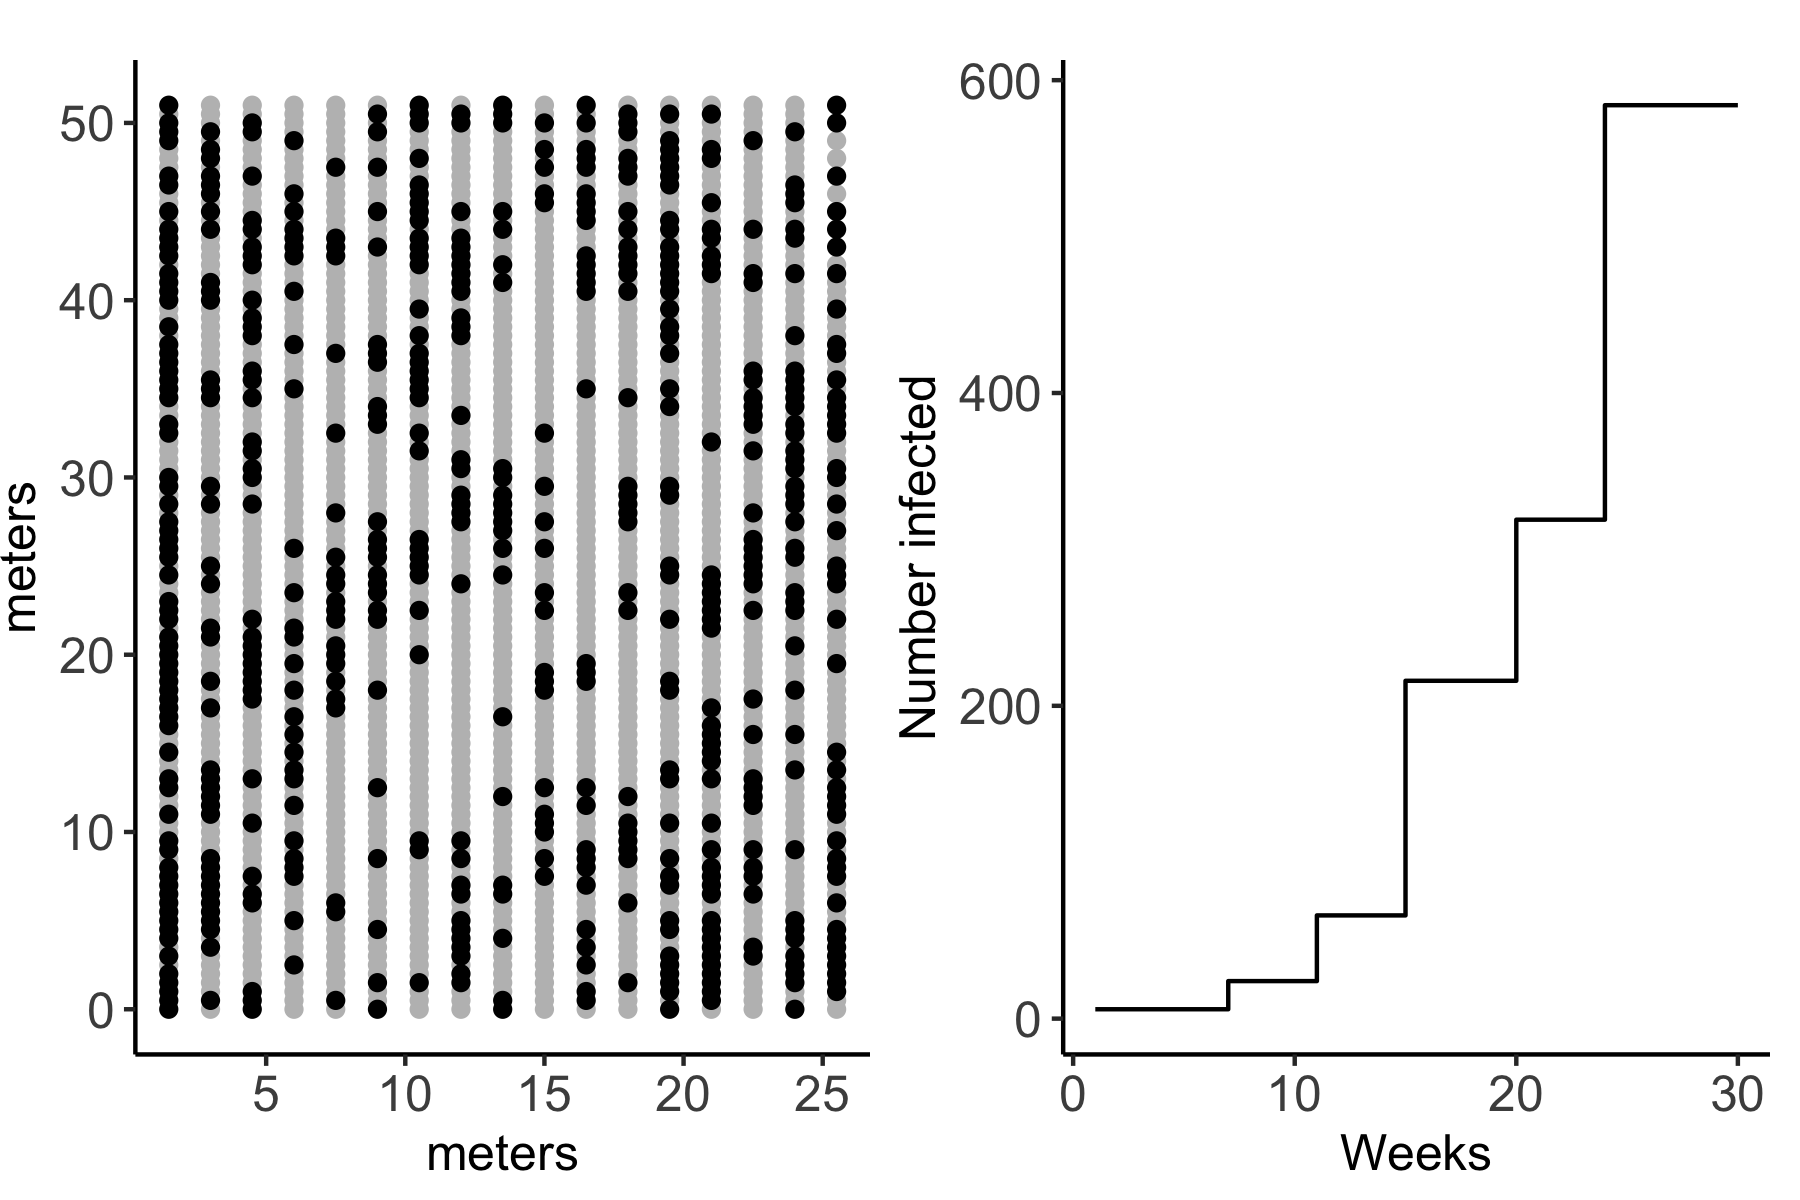
\includegraphics[height=0.45\linewidth, keepaspectratio]{figures/figure_1.png}
\caption{Replicated Figure 1}
   \label{fig:data_plot}
\end{figure}

\vmcomment{Add axis labels to the left plot: ``grid dimension 1" and ``grid dimension 2".} 
Figure \ref{fig:data_plot} summarizes the sugar cane data set. The black dots indicate locations of infected plants at the conclusion of the 30 week study period. Grey dots indicate the location of plants that were not infected. The plot on the right shows the cumulative number of infected plants for each inspection. 

\section{Methods}
\subsection{Model and Likelihood}
\v
Inference for ILM model parameters begins with the likelihood function. 
Plausible models account for the locations of infected and susceptible plants along with the respective infection times and durations of exposures. 
However, time intervals in which a susceptible plant becomes infected offer the only temporal queues. 
As a result, infection time, $\tau_j$, for plant $j$ is treated as a latent variable. 

The model must also account for the transmission rate differential induced by the physical distance separating infected and susceptible plants. 
The transmission rate between an infected plant far from a susceptible plant should be smaller than the rate between two plants next to one another.
As a result, let the function $\theta f(x_i -x_j \sigma | \sigma)$ dente the rate of infection for plant $i$ at time $t$ and for a plant $j$ infected prior to $t$. 
Accounting for the rate of spontaneous infection $\mu$, the cumulative intensity of infections at plant $i$ and time $t$ given the infection times for plants $j \in \{1, 2, \dots, 1742\}$ is 

\vmcomment{Try to rewrite it now with CTMC generating process.}

$$ \lambda(x_i,t) = \mu + \sum_{j; \tau_j<t} \theta \, f(x_i - x_j; \sigma)$$\vmadd{.}

While this function increases with time, the SI construct assumed for these data suggest that once a plant becomes infected, it remains infected. 
With the rate of infection established, the likelihood of observing infection times $\{\tau_1, \dots, \tau_N\}$ becomes
\begin{itemize}
\item Probability of not observing infections during each plant's time in the susceptible state 
\item Probability of observing infections at each $\tau_i$
\end{itemize}
Approximating infection events with a Poisson process and noting that the rate parameter equals the mean, the probability that plant $i$ remains uninfected up to time $\tau_i$ is 
$$ \exp \left\{- \int^{\tau_i}_{0} \lambda(x_i, u) du \right\}$$
The density function associated with an infection at time $\tau_i$, $\lambda(x_i, \tau_i)$, is the second component of the likelihood. 
The probability that a plant remains uninfected throughout the period under consideration follows the same Poisson process reasoning used as above. 
This leads to the following likelihood equation. 
\begin{equation} L_{\theta, \mu, \tau} \propto \left[ \prod_{i;\tau_i \le T} \exp \left\{-\int^{\tau_i}_0 \lambda(x_i, t)dt\right \} \lambda(x_i, \tau_i)\right] \left\{ \prod_{i;\tau_i > T} \exp \left\{-\int^{\tau_i}_0 \lambda(x_i, t)dt\right \}\right\} \end{equation}

It remains to specify the infection kernel function, $f(x_i -x_j \sigma | \sigma)$. In this case, a radially symmetric bivariate Gaussian density is appropriate. 
\begin{equation} f(d|\sigma) = \frac{1}{\sqrt{2\pi \sigma^2}} \exp \left\{-\frac{||d||^2}{2\sigma^2} \right\} \label{eq:kernel} \end{equation}
\cite{Brown} reasons that the Gaussian kernel is appropriate considering the movement of amphids is Brownian Motion. 
With that argument, $\sigma^2$ in (\ref{eq:kernel}) denotes the variance of the distance an amphid travels in one week. 

\subsection{Prior Distributions}
Weakly informative priors were used for the endemic infection rate ($\mu$), the epidemic infection rate ($\theta$), and the variance for distance disease travels in a week ($\sigma^2$). 
Prior parameters were specified by considering the 95\% prediction intervals considering on the number of infections observed over 30 weeks time.
In particular,  
\begin{itemize}
\item $\mu \sim$ Gamma(0.7, 0.004) yields a 95\% prediction interval between 1 and 630. 583 infections were observed in the data.
\item $\theta \sim$ Gamma(0.8, 10) leads to an infected plant requiring 1 to 16 weeks time to produce the first infection when surrounded by susceptible plants
\item $\sigma \sim$ Gamma(0.5, 100) implies that nearly all amphids will have traveled less than 10 cm at the 2.5\% quantile and around 500 meters at the 95.5\% quantile
\end{itemize}
Placing $\mu$ and $\theta$ at the lower end of their ranges leads to few infections over 30 weeks time. 
Setting these too high leads to nearly universal infection. 
Extreme values of $\sigma$ leads a to somewhat different result. 
Specifying $\sigma$ too small would imply that the amphids driving the infection spread are incapable of moving between plants. 
Setting $\sigma$ too large removes the spatial component of the model. 
\cite{Brown} specified priors leading to physically plausible outcomes. 


\subsection{Inference}
Exact infection times, $\tau_i$, are unobserved. 
Only the intervals in which a plant became infected offer clues about the status of plants during the study period. 
Since each plant's infection status and location influence all other plants at each time step, there is no way to eliminate the dependency on the unknown infection times, $\tau$.
\cite{Brown} follows a data augmentation and MCMC approach to resolve handle the issue. 
This process is known as a \textit{non-centering parameterization} in the literature and \cite{Jewell} section 2.2 outlines a modeling framework nearly identical to the methods followed here. 

In this case, priors are specified for the model parameters of interest, specifically $\theta$, $\sigma$, and $\mu$. 
Infection intervals, $\textbf{Y} = \{Y_i:i=1,\dots, N\}$, are the data. 
The Metropolis algorithm summarized below leads to a posterior sample from $\pi(\mu, \theta, \sigma, \tau \mid \textbf{Y})$. 

\begin{enumerate}
\item Initialize the algorithm at $\tau_i^{0}$, $\mu^{0}$, $\sigma^{0}$, $\theta^{0}$ for iteration $r=0$
\item at iteration $r$, set $\tau_i^{(r)}=\tau_i^{(r-1)}$, $\mu^{(r)}=\mu^{(r-1)}$, $\sigma^{(r)}=\sigma^{(r-1)}$, $\theta^{(r)}=\theta^{(r-1)}$
\item simulate a proposal $\mu^{\star} \sim N(\mu^{(r-1)}, \nu_{\mu})$
\item set $\mu^{(r)} = \mu^{\star}$ with probability
$$\min \left\{1, \frac{L( \tau^{(r)}_1, \dots, \tau^{(r)}_N \mid \mu^{\star}, \theta^{(r)}, \sigma^{(r)} ) \; p_{\mu}(\mu^{\star})}{L(\tau^{(r)}_1, \dots, \tau^{(r)}_N \mid \mu^{(r)}, \theta^{(r)}, \sigma^{(r)} ) \; p_{\mu}(\mu^{r})} \right\} $$
			otherwise, set $\mu^{(r)}=\mu^{(r-1)}$
\item repeat steps 3 and 4 for $\theta$ and $\sigma$
\item for each $i=1, \dots, N$, propose a new $\tau^{\star}_i$ and accept with probability
$$\min \left\{1, \frac{L( \tau^{(r)}_1, \dots, \tau^{(r)}_{i-1}, \tau^{\star}_i,\tau^{(r)}_{i+1}, \dots, \tau^{(r)}_N \mid \mu^{(r)}, \theta^{(r)}, \sigma^{(r)} ) \; p_{\mu}(\mu^{\star})}{L(\tau^{(r)}_1, \dots, \tau^{(r)}_N \mid \mu^{(r)}, \theta^{(r)}, \sigma^{(r)} ) \; p_{\mu}(\mu^{r})} \right\} $$
\item return to step 2 until a sufficiently large sample has been obtained
\end{enumerate}

The implementation for this model uses normally distributed proposals with means at the previous $\theta$, $\sigma$, $\mu$, and $\tau_i$ values and $ \nu_{\theta}=0.005^2$, $ \nu_{\mu}=0.0005^2$, $ \nu_{\sigma}=0.05^2$, and $ \nu_{\tau^{(r)}_i}=1$. 
The authors select these standard deviations after assessing the mixing properties of test runs. 

\subsection{Implementation}
The data include 583 unknown infection times. 
As a result, some portion of the likelihood function has to be computed 586 times for each pass through the sampler. 
Implementing the algorithm naively leads to prohibitively long computation times. 
The following sections review the steps taken to improve and benchmark computational performance enough to make the non-centering parameterization method viable for data with challenging interdependencies. 
The methods were implemented in the Julia. 

\subsubsection{Basic Algorithm}
The basic implementation primarily executes the pseudo-code from the previous section with three exceptions.
First, the distance matrix among the 1,742 plants is pre-computed and referenced throughout the implementation. 
The other exception concerns the $\tau^{(r)}$ update routine. 
Many of the terms in the likelihood ratio are identical, eliminating the need to compute several terms in the likelihood function. 
Finally, eliminating impossible infection time sequences among the remaining pieces of the computation led to efficiencies in the compute time.

\subsubsection{Parallel Algorithm}
The parallel implementation distributes the computational burden two different ways. 
Both focus on computing updating $\tau$. 
First, the subroutines of the likelihood ratio that cannot run asynchronously but still require significant computational resources are broken into pieces and computed on multiple cores. 
The other parallelization improvement results from recognizing that some updates are not possible given order that infections were known to have occurred. 
As a result, proposals that would reverse this known ordering are rejected immediately. 
More to come... 

\subsubsection{Improved Parallel Algorithm}
Tbd...

\subsubsection{Truncated Algorithm}
Tbd...

\subsubsection{Discrete Time Algorithms}
Tbd...

\section{Results}

\section{Discussion}

\bibliography{prelim_references}

\end{document}









